\pagebreak
\section{Resultados}

\subsection{Imagenes originales}

En la figura \ref{fig:normal_results} se observan los resultados obtenidos por el modelo con las diferentes maneras de entrenamiento.

\begin{figure}[H]
    \centering
    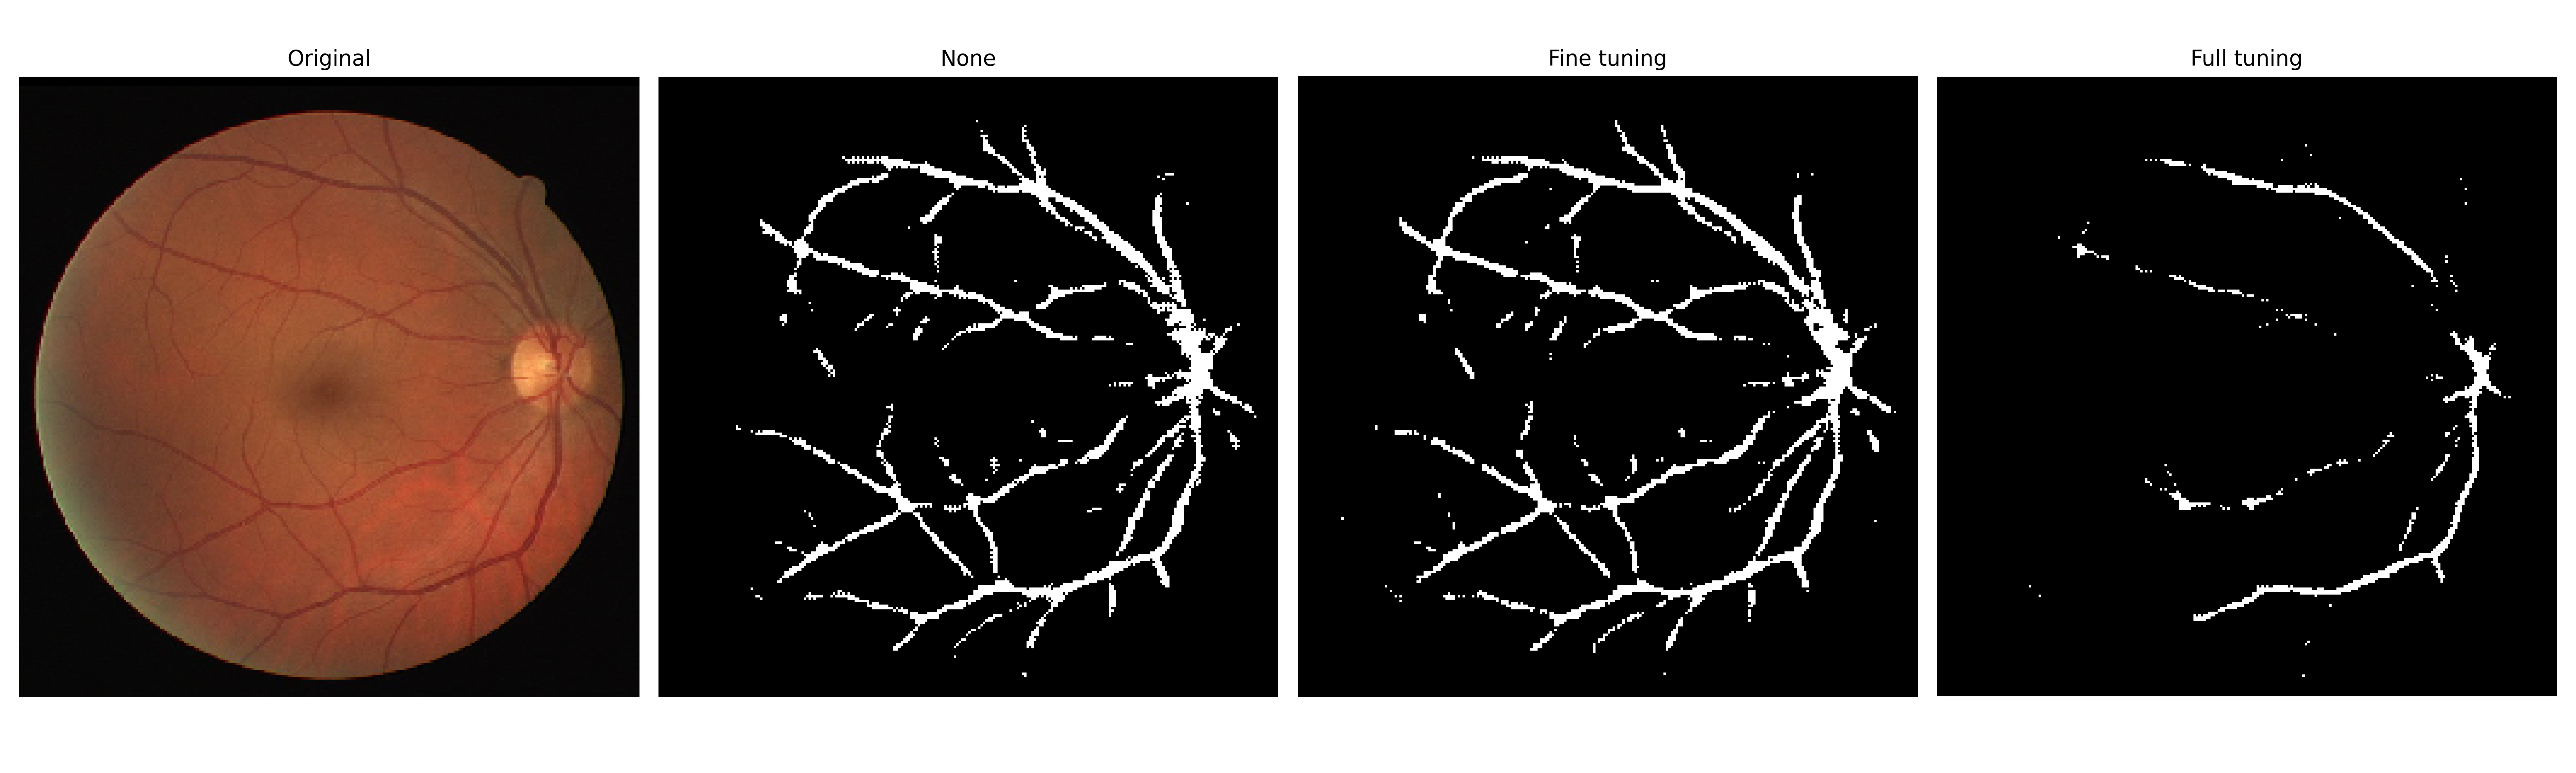
\includegraphics[width=14cm]{Graphics/normal/04.png}
    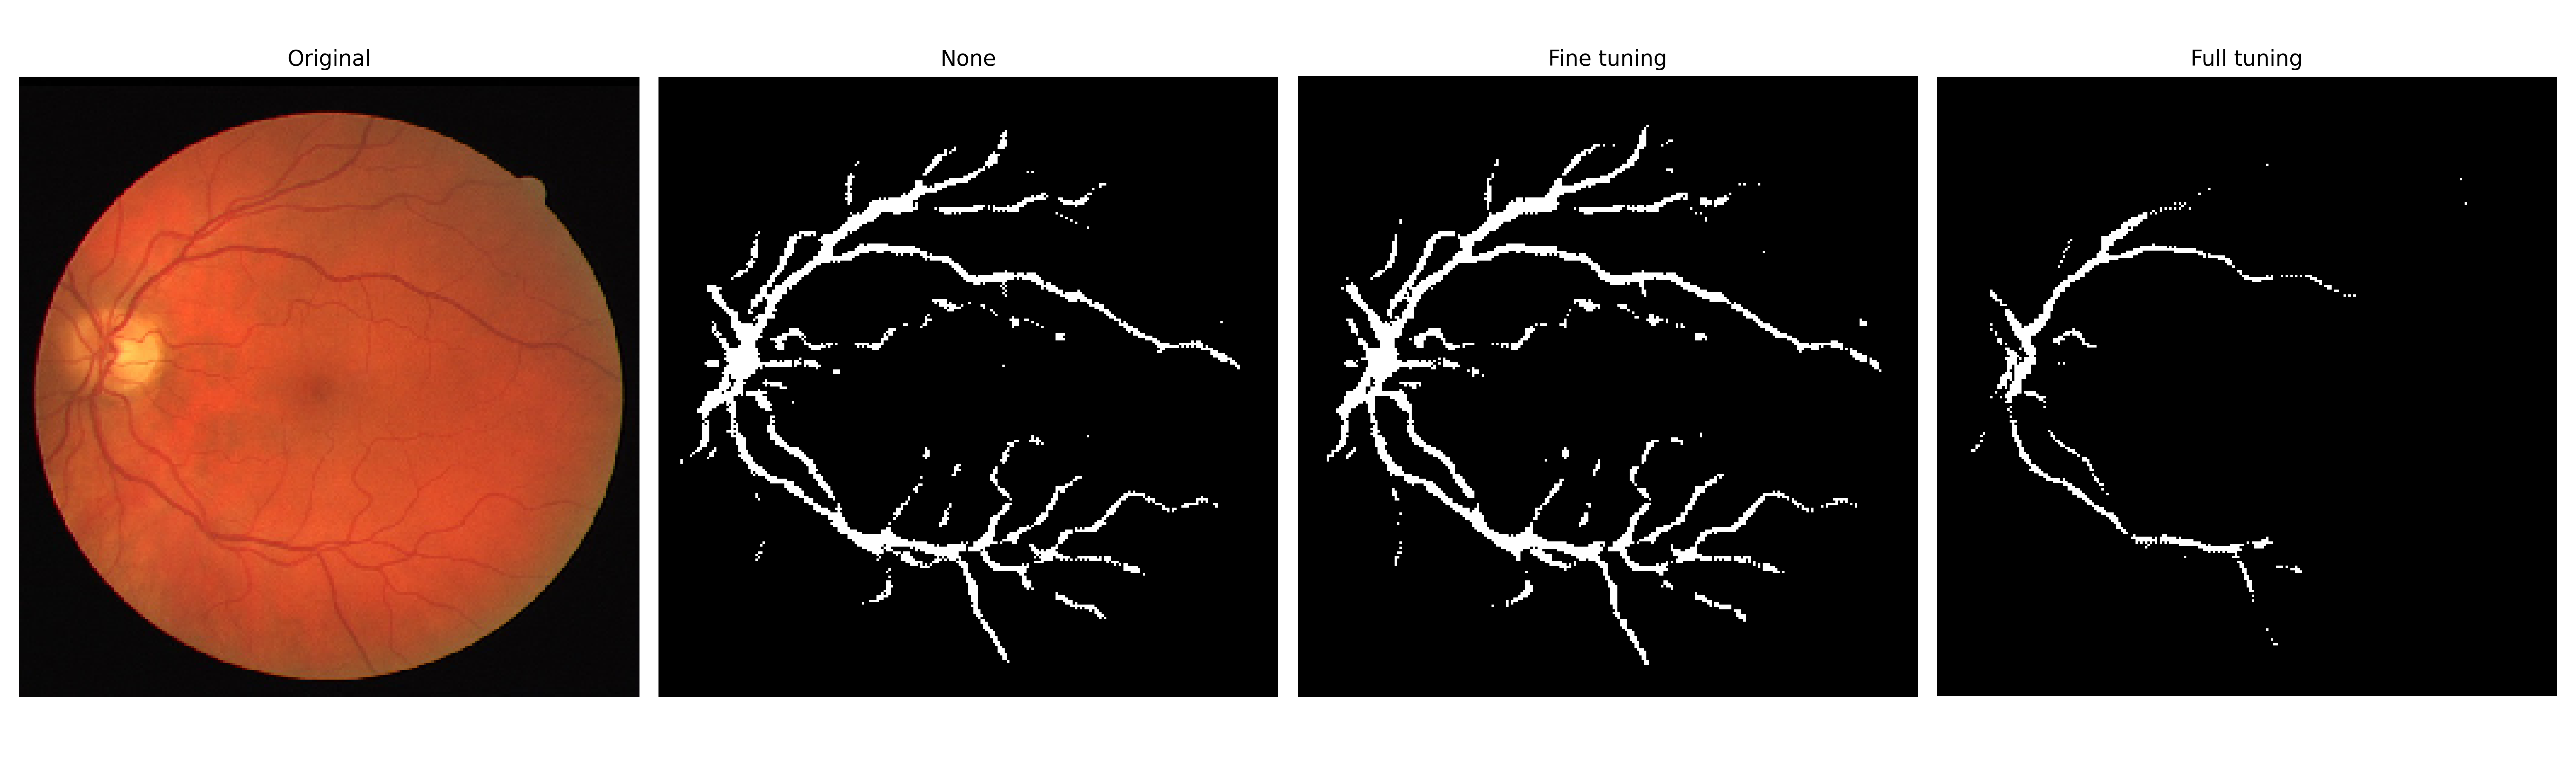
\includegraphics[width=14cm]{Graphics/normal/06.png}
    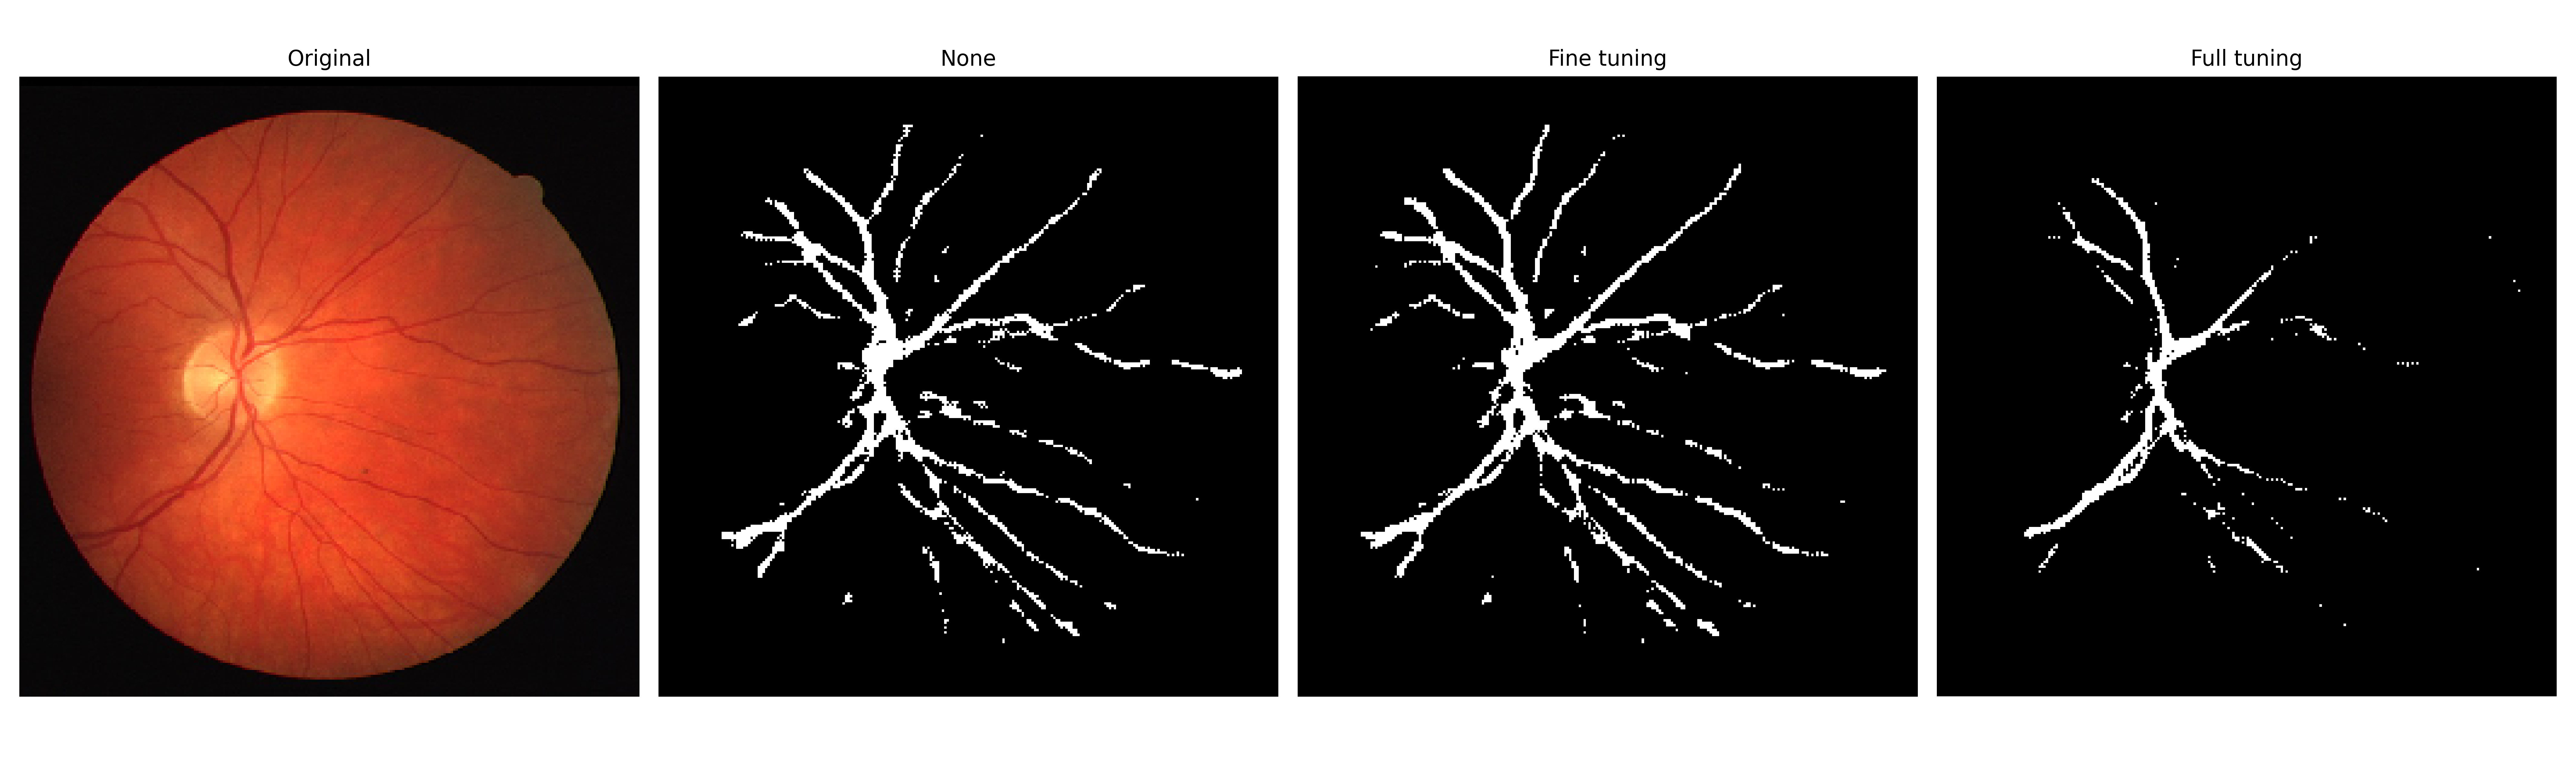
\includegraphics[width=14cm]{Graphics/normal/10.png}
    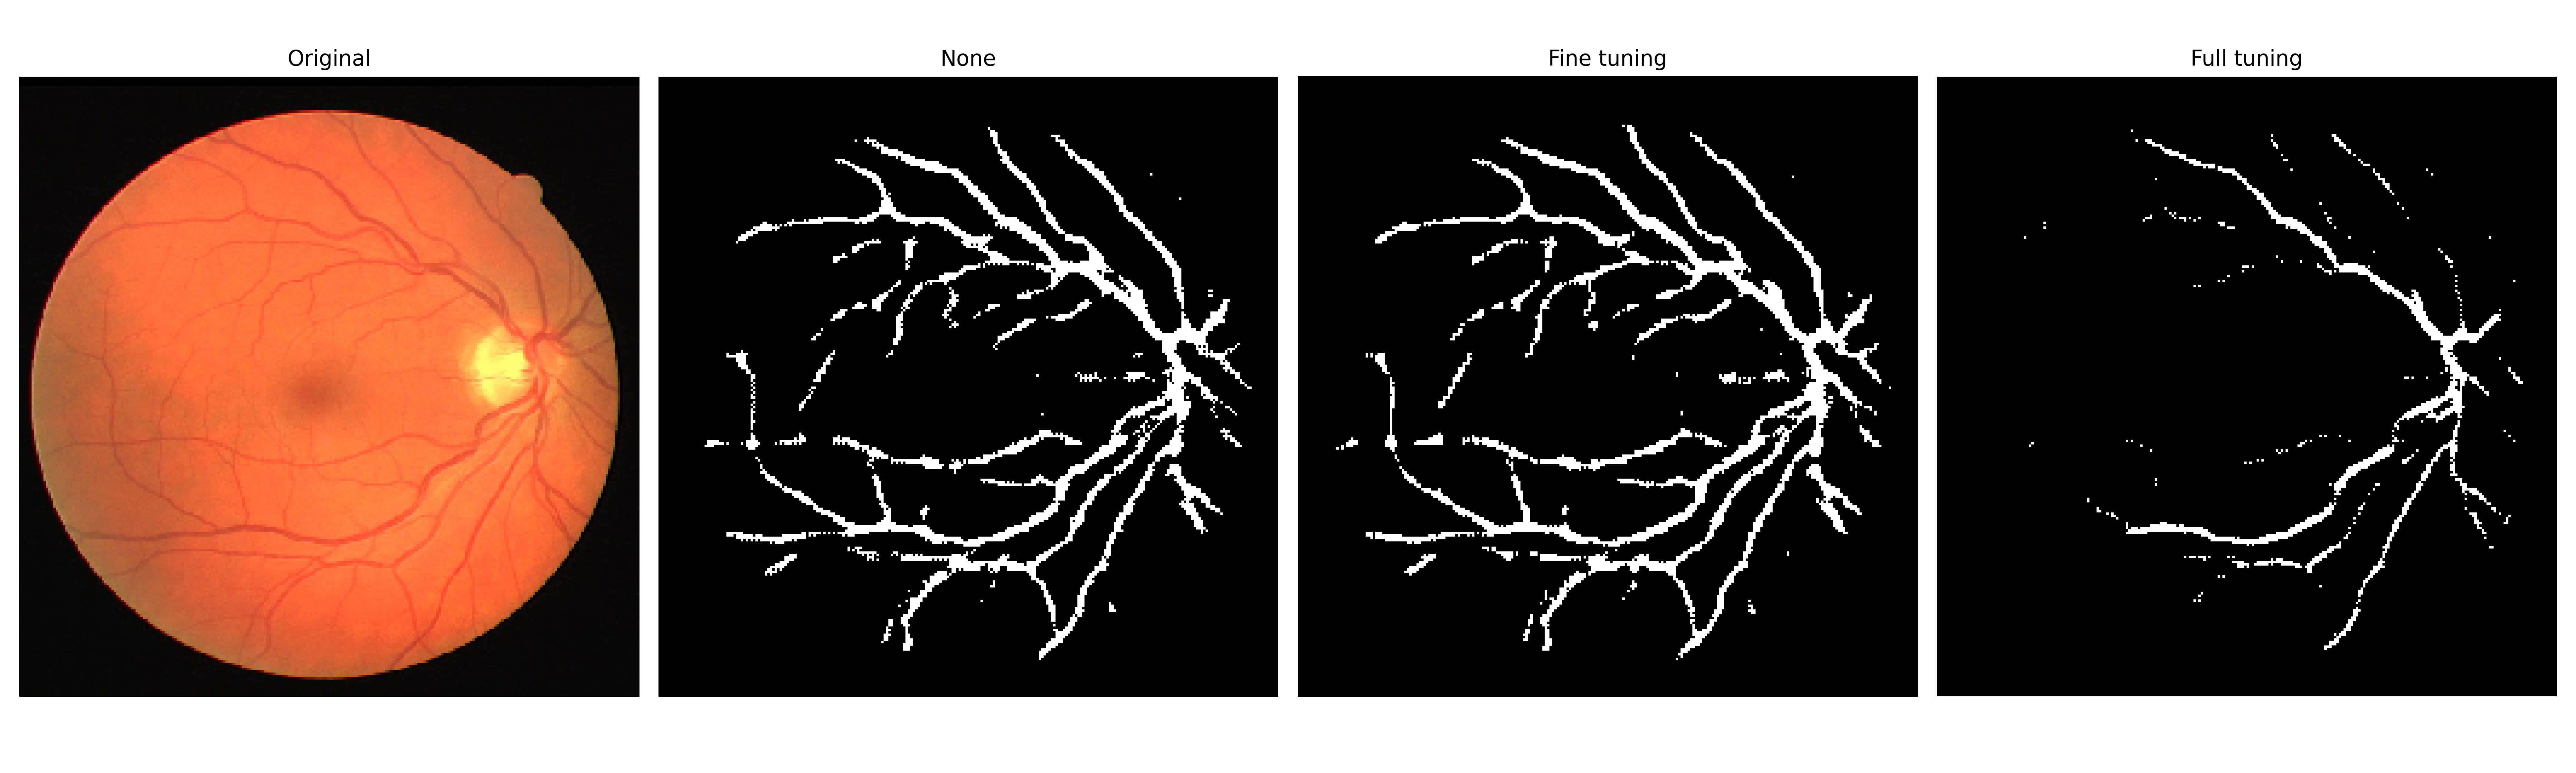
\includegraphics[width=14cm]{Graphics/normal/14.png}
    \caption{Resultados para una muestra del conjunto de prueba con los diferentes modelos usando como entrada las imágenes originales.}
    \label{fig:normal_results}
\end{figure}

\subsection{Imágenes con alto contraste}

En la figura \ref{fig:high_contrast_results} se observan los resultados obtenidos por el modelo con las diferentes maneras de entrenamiento.

\begin{figure}[H]
    \centering
    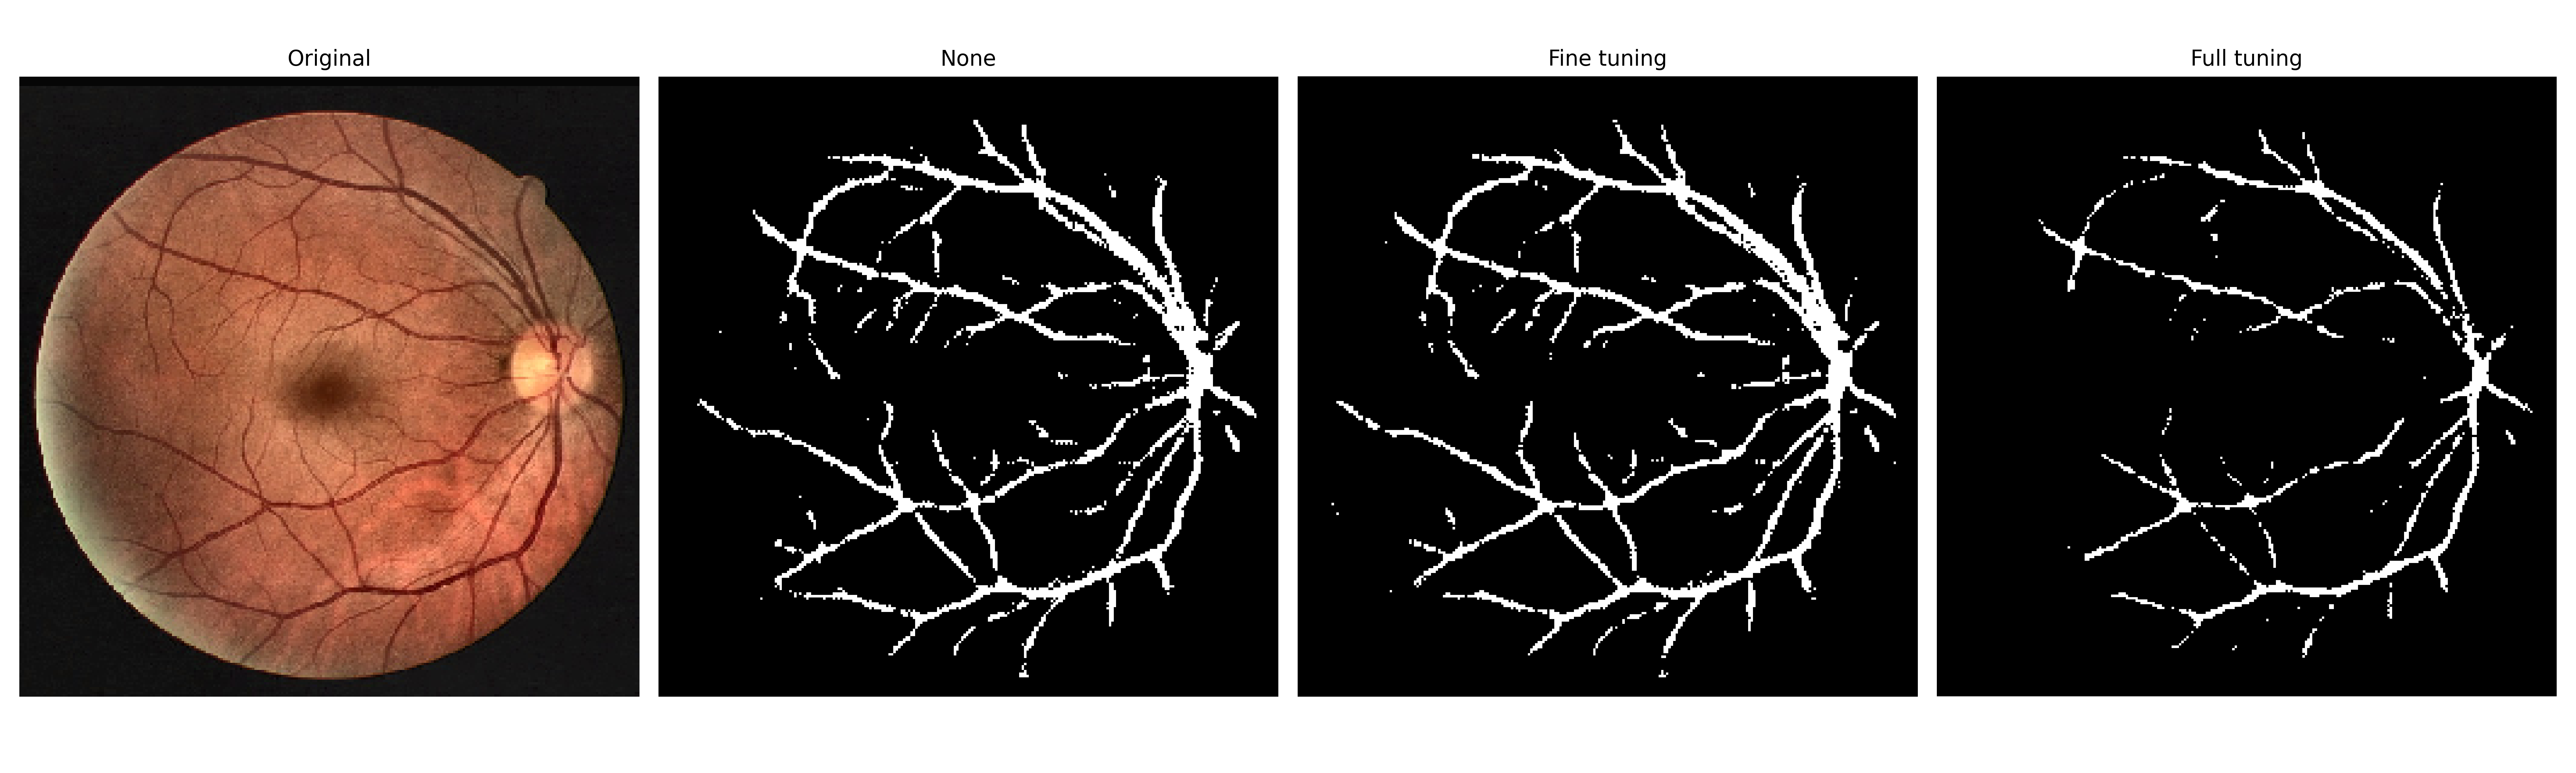
\includegraphics[width=14cm]{Graphics/high_contast/04.png}
    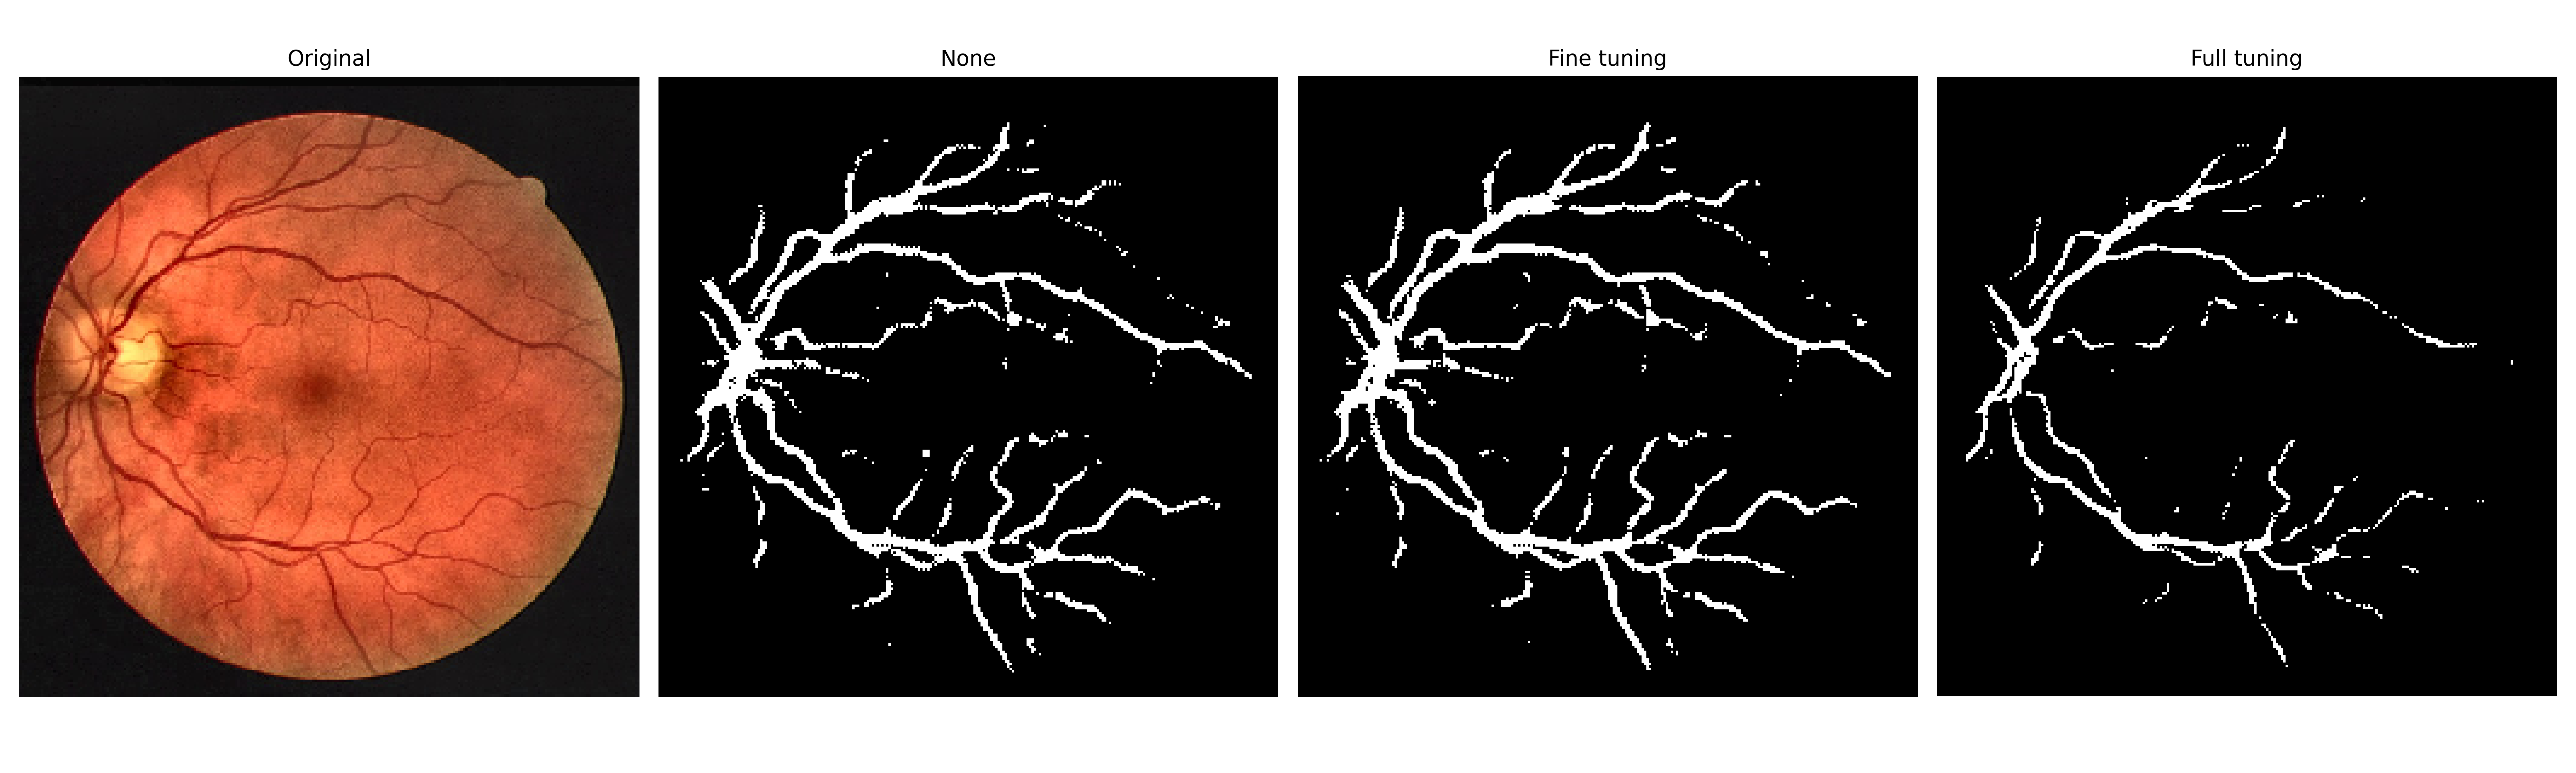
\includegraphics[width=14cm]{Graphics/high_contast/06.png}
    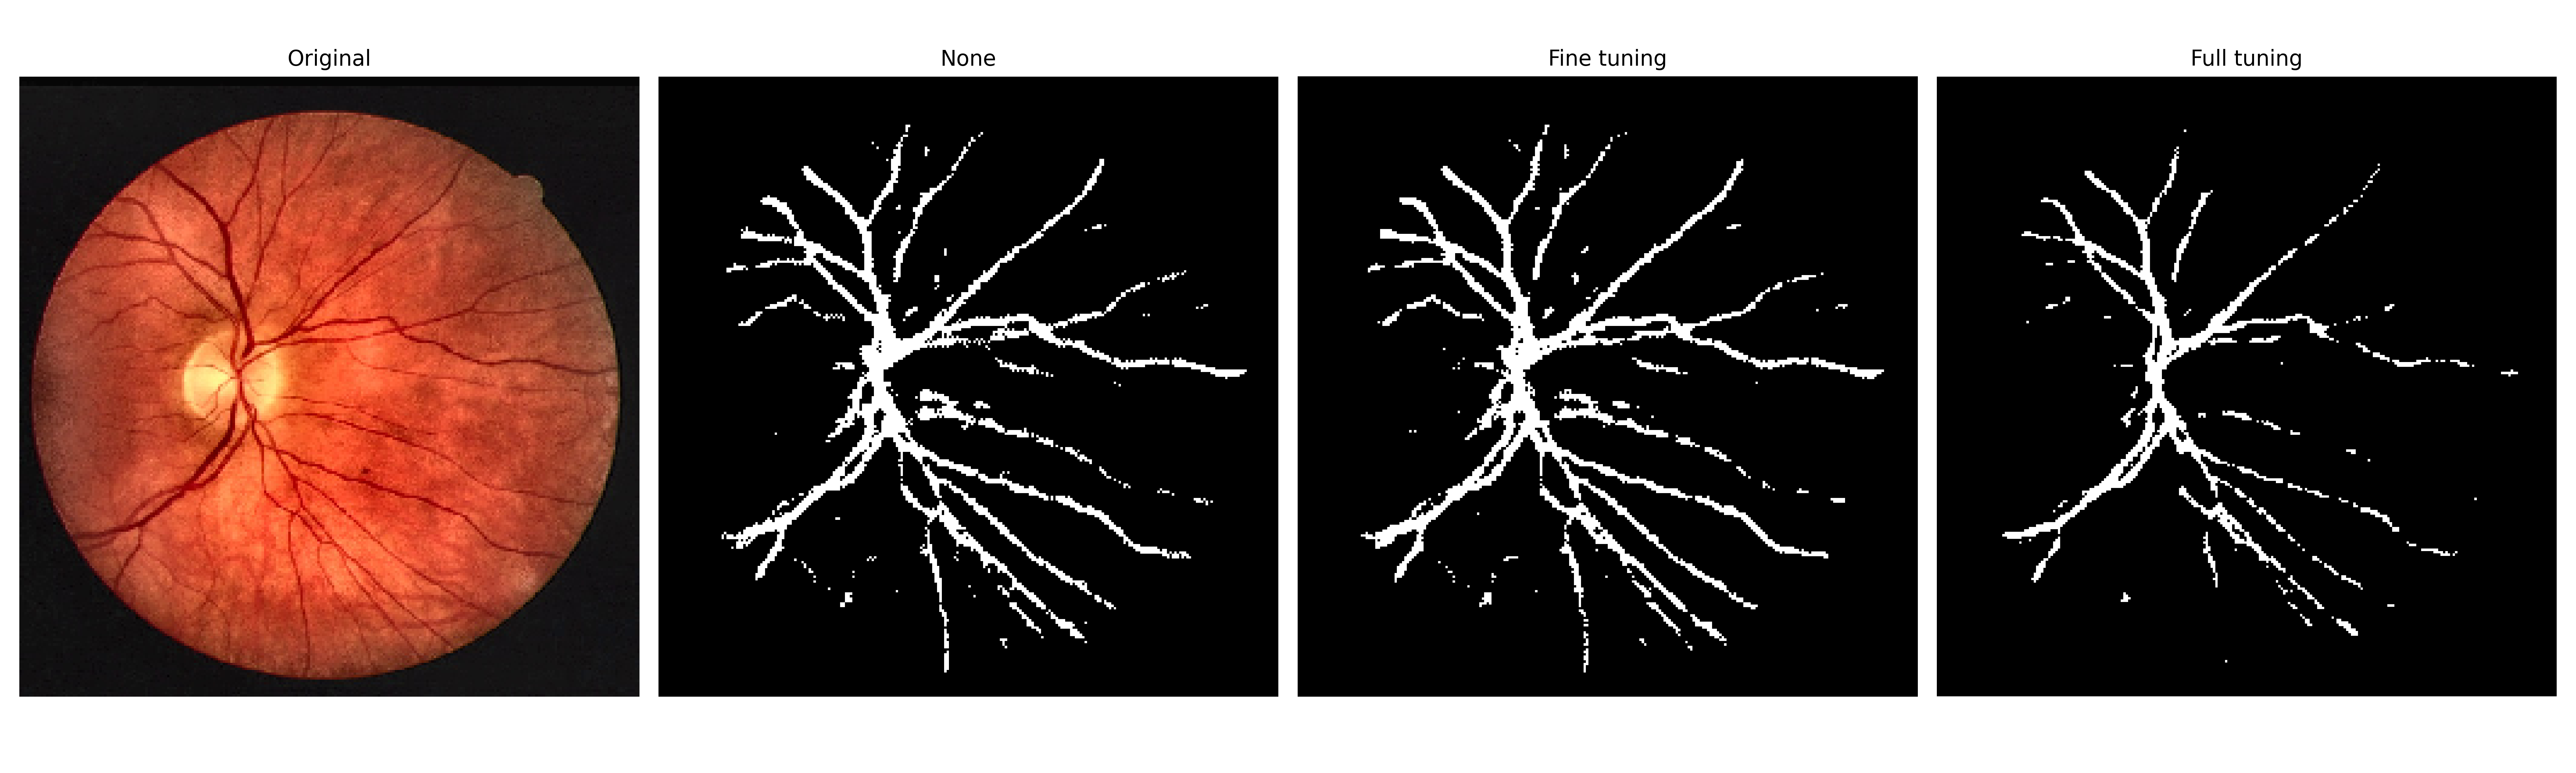
\includegraphics[width=14cm]{Graphics/high_contast/10.png}
    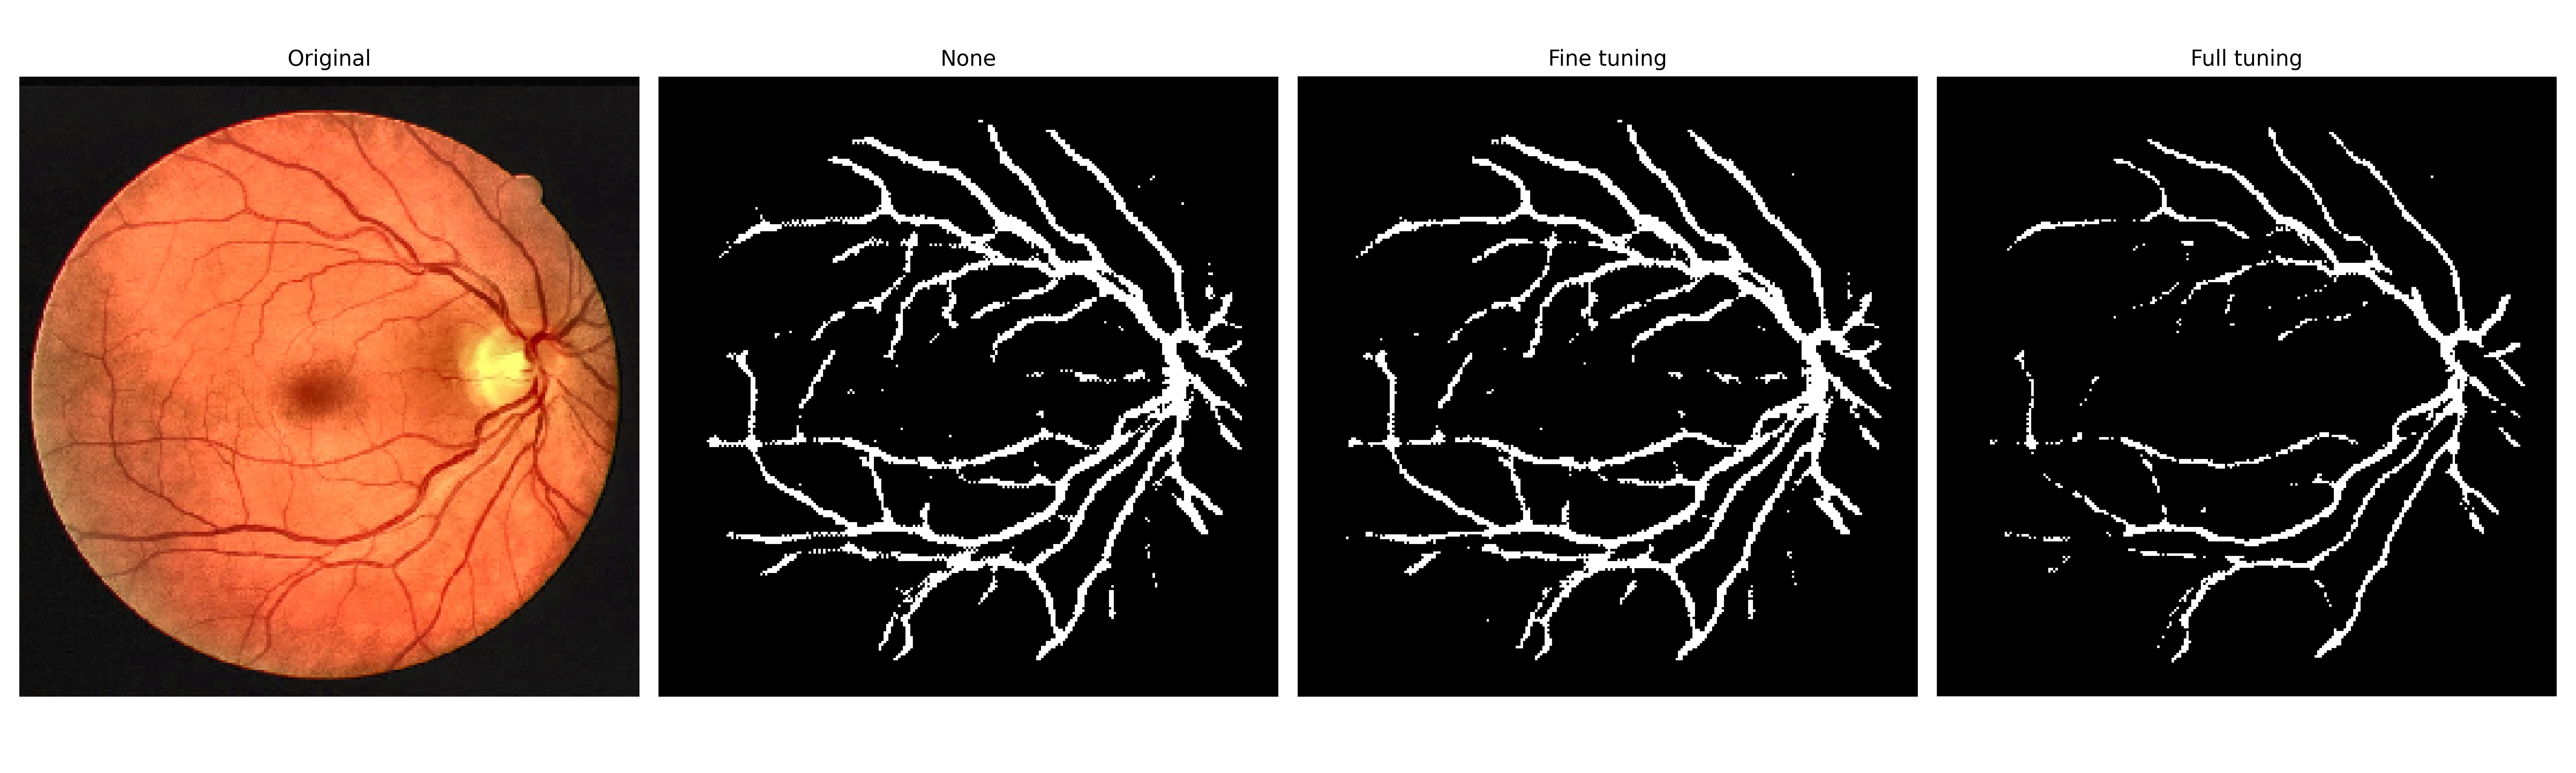
\includegraphics[width=14cm]{Graphics/high_contast/14.png}
    \caption{Resultados para una muestra del conjunto de prueba con los diferentes modelos usando como entrada las imágenes con el filtro de alto contraste.}
    \label{fig:high_contrast_results}
\end{figure}


\subsection{Imágenes en escala de grises}

En la figura \ref{fig:grayscale} se observan los resultados obtenidos por el modelo con las diferentes maneras de entrenamiento.

\begin{figure}[H]
    \centering
    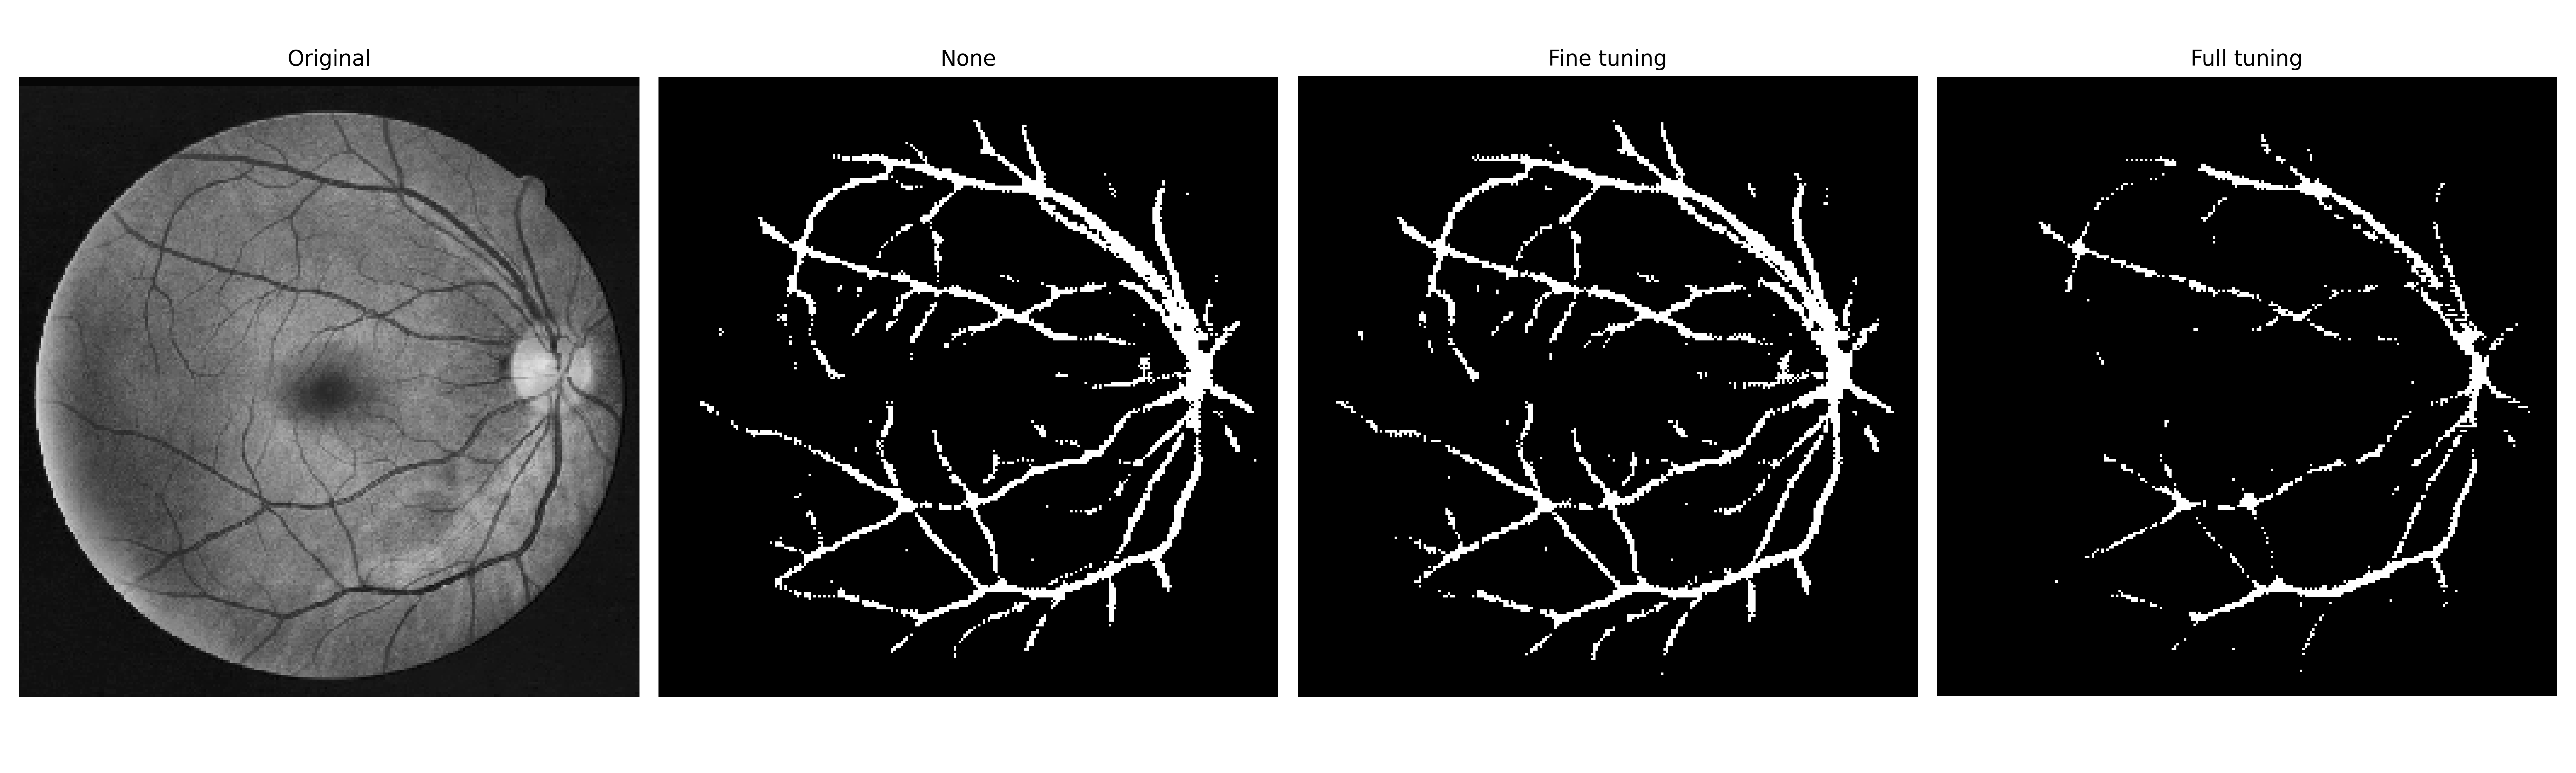
\includegraphics[width=14cm]{Graphics/grayscale/04.png}
    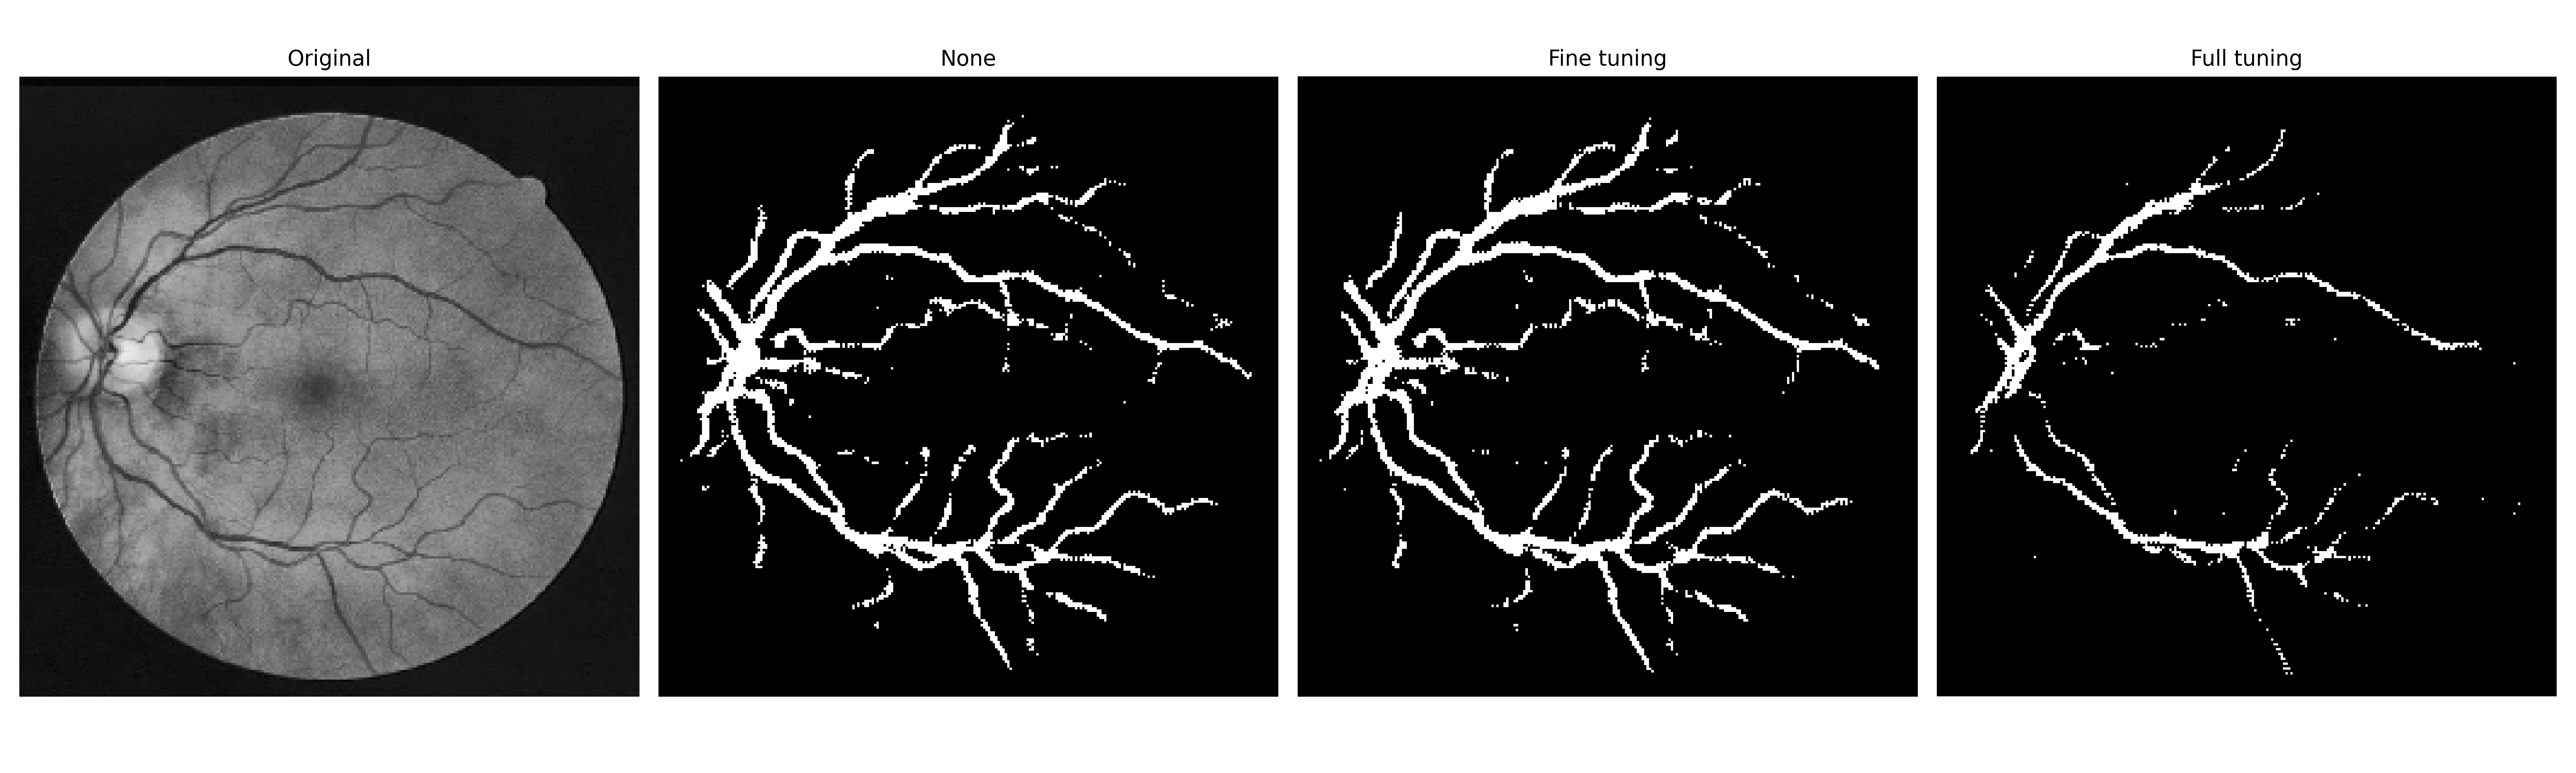
\includegraphics[width=14cm]{Graphics/grayscale/06.png}
    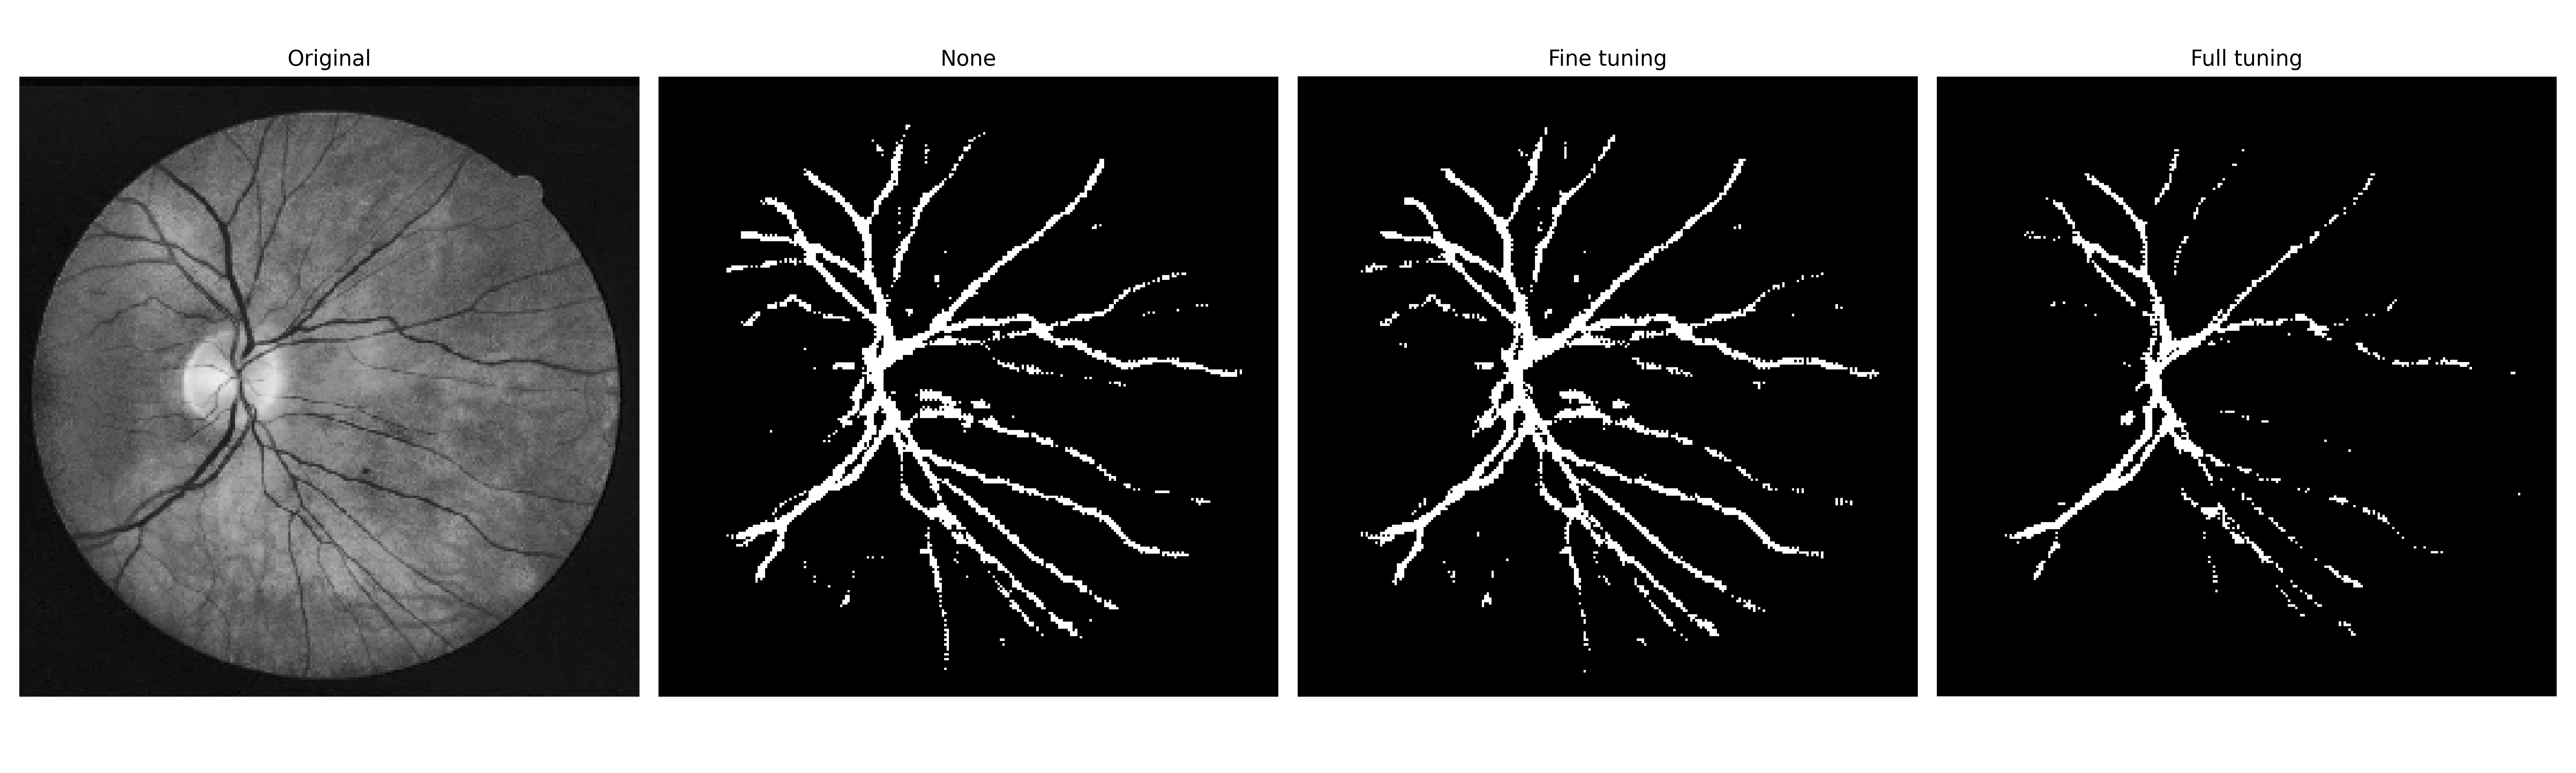
\includegraphics[width=14cm]{Graphics/grayscale/10.png}
    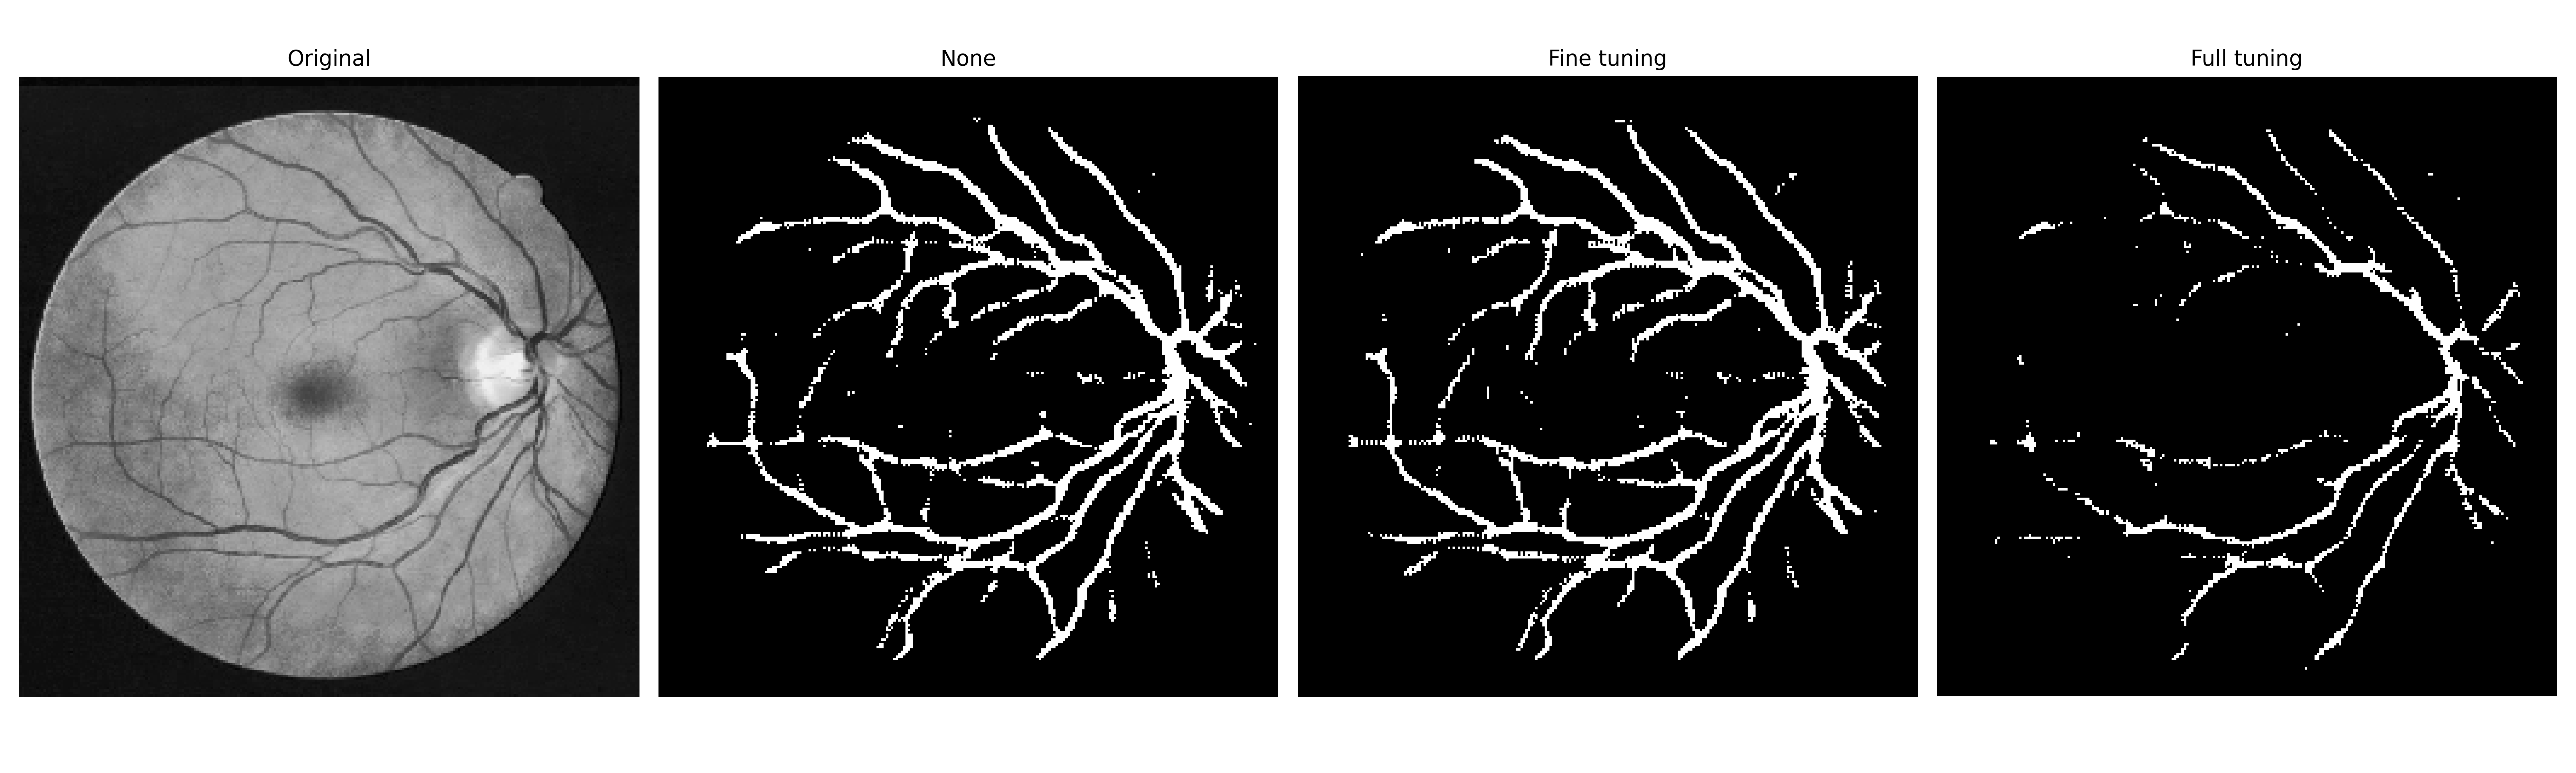
\includegraphics[width=14cm]{Graphics/grayscale/14.png}
    \caption{Resultados para una muestra del conjunto de prueba con los diferentes modelos usando como entrada las imágenes en escala de grises.}
    \label{fig:grayscale_results}
\end{figure}
